\documentclass[10pt,twocolumn,letterpaper]{article}

\usepackage{iccv}
\usepackage{times}
\usepackage{epsfig}
\usepackage{graphicx}
\usepackage{amsmath}
\usepackage{amssymb}

\DeclareMathOperator{\iou}{IoU}
\DeclareMathOperator*{\argmax}{arg\,max}

% Include other packages here, before hyperref.

% If you comment hyperref and then uncomment it, you should delete
% egpaper.aux before re-running latex.  (Or just hit 'q' on the first latex
% run, let it finish, and you should be clear).
\usepackage[breaklinks=true,bookmarks=false]{hyperref}

\iccvfinalcopy % *** Uncomment this line for the final submission

\def\iccvPaperID{****} % *** Enter the ICCV Paper ID here
\def\httilde{\mbox{\tt\raisebox{-.5ex}{\symbol{126}}}}

% Pages are numbered in submission mode, and unnumbered in camera-ready
\ificcvfinal\pagestyle{empty}\fi

\begin{document}

%%%%%%%%% TITLE
\title{Stelynx Optical Flow-based Object Tracker for Steady Environments}

\author{Marcel Campa\\
University of Ljubljana, Faculty of Electrical Engineering\\
Trzaska cesta 25, 1000 Ljubljana, Slovenia\\
{\tt\small marcel@stelynx.com}
}

\maketitle
% Remove page # from the first page of camera-ready.
\ificcvfinal\thispagestyle{empty}\fi

%%%%%%%%%%%%%%%%%%%%%%%%%%%%%%%%%%%%%%%%%%%%%%%%%%%%%%%%%%%%%%%%%%%%%%%%%%%%%%%%%%%%%%%%%%%%%%%%
%%%%%%%%%%%%%%%%%%%%%%%%%%%%%%%%%%%%%%%%%%%%%%%%%%%%%%%%%%%%%%%%%%%%%%%%%%%%%%%%%%%%%%%%%%%%%%%%
%%%%%%%%%
%%%%%%%%% ABSTRACT
%%%%%%%%%
%%%%%%%%%%%%%%%%%%%%%%%%%%%%%%%%%%%%%%%%%%%%%%%%%%%%%%%%%%%%%%%%%%%%%%%%%%%%%%%%%%%%%%%%%%%%%%%%
%%%%%%%%%%%%%%%%%%%%%%%%%%%%%%%%%%%%%%%%%%%%%%%%%%%%%%%%%%%%%%%%%%%%%%%%%%%%%%%%%%%%%%%%%%%%%%%%

\begin{abstract}
   Tracking multiple objects is essential for any autonomous vehicle in order for the
   system to be able to estimate the future trajectory of the tracked objects.
   By having a knowledge of its surroundings, an autonomous vehicle can interact
   with or react ot the movement of surrounding objects, giving it an ability
   to plan their actions in the subject's environment, e.g. plan route or evade
   obstacles.

   This paper presents a state-of-the-art technique for
   multiple object tracking in steady environments, like maritime environment. The proposed
   method is based on optical flow and does not require any pretraining. Due to
   its lightweightness it is highly usable in embedded systems like unmanned aerial
   vehicles (UAVs) or unmanned surface vehicles (USVs).
\end{abstract}


%%%%%%%%%%%%%%%%%%%%%%%%%%%%%%%%%%%%%%%%%%%%%%%%%%%%%%%%%%%%%%%%%%%%%%%%%%%%%%%%%%%%%%%%%%%%%%%%
%%%%%%%%%%%%%%%%%%%%%%%%%%%%%%%%%%%%%%%%%%%%%%%%%%%%%%%%%%%%%%%%%%%%%%%%%%%%%%%%%%%%%%%%%%%%%%%%
%%%%%%%%%
%%%%%%%%% INTRODUCTION
%%%%%%%%%
%%%%%%%%%%%%%%%%%%%%%%%%%%%%%%%%%%%%%%%%%%%%%%%%%%%%%%%%%%%%%%%%%%%%%%%%%%%%%%%%%%%%%%%%%%%%%%%%
%%%%%%%%%%%%%%%%%%%%%%%%%%%%%%%%%%%%%%%%%%%%%%%%%%%%%%%%%%%%%%%%%%%%%%%%%%%%%%%%%%%%%%%%%%%%%%%%

\section{Introduction}

Autonomous vehicles are closer and closer to reality. In order for them to be able to
autonomously navigate in their respective environments, they must be able to detect and
in many cases track objects in their surroundings.

Such systems require power to operate and general-use computers require an enormous
ammount of it making them unusable for autonomous vehicles using batteries or solar panels
as their power sources. Not to mention that computers are heavy. Therefore, such
autonomous vehicles often use embedded hardware, trading computing power for lower
weight and less energy consumption. One can see the importance of simple and lightweight
algorithms that can run in real-time on embedded systems.

This work presents a simple yet powerful object tracker that can easily run on embedded
hardware in zero-to-no delay. The algorithm presented is most suitable for use in
environments in which objects move slowly inside a single-frame time period, which is
especially true for maritime, aerial and rural environments, but also holds for not so crowded
urban environments.


%%%%%%%%%%%%%%%%%%%%%%%%%%%%%%%%%%%%%%%%%%%%%%%%%%%%%%%%%%%%%%%%%%%%%%%%%%%%%%%%%%%%%%%%%%%%%%%%
%%%%%%%%%%%%%%%%%%%%%%%%%%%%%%%%%%%%%%%%%%%%%%%%%%%%%%%%%%%%%%%%%%%%%%%%%%%%%%%%%%%%%%%%%%%%%%%%
%%%%%%%%%
%%%%%%%%% RELATED WORK
%%%%%%%%%
%%%%%%%%%%%%%%%%%%%%%%%%%%%%%%%%%%%%%%%%%%%%%%%%%%%%%%%%%%%%%%%%%%%%%%%%%%%%%%%%%%%%%%%%%%%%%%%%
%%%%%%%%%%%%%%%%%%%%%%%%%%%%%%%%%%%%%%%%%%%%%%%%%%%%%%%%%%%%%%%%%%%%%%%%%%%%%%%%%%%%%%%%%%%%%%%%

\section{Related Work}

There are many different approaches to object tracking \cite{1195991,bewley2016simple,wojke2017simple,mahmoudi2019multi,fortmann1980multi,girshick2015fast}.
We can classify them into two broad categories, those using deep-learning methods like convolutional
neural networks (CNNs) and those that do not use any machine learning techniques. Our work does not
make use of any machine learning method, therefore we omit these algorithms from consideration.

The most notable object tracking algorithm that does not make use of deep learning is SORT \cite{bewley2016simple}.
It first uses Kalman filter \cite{welch1995introduction} to predict future locations of objects tracked,
computes overlaps between detected objects in future frames to produce correction, and finally
maps detections using Hungarian algorithm for the assignment problem \cite{kuhn1955hungarian}.

Another notable object tracking algorithm that outperforms the rest based on frames-per-second (FPS) processed
is the IOU Tracker \cite{8078516}. The algorithm is a simpler method than what we propose in this
paper, because all it does is explores area close to bounding box from previous frame and finds
a new bounding box using intersection over union (IoU) measure. The IOU Tracker algorithm
achieves over 100K frames-per-second processed. Our proposed method is more robust and it takes
image information into account, whereas IOU Tracker does not.


%%%%%%%%%%%%%%%%%%%%%%%%%%%%%%%%%%%%%%%%%%%%%%%%%%%%%%%%%%%%%%%%%%%%%%%%%%%%%%%%%%%%%%%%%%%%%%%%
%%%%%%%%%%%%%%%%%%%%%%%%%%%%%%%%%%%%%%%%%%%%%%%%%%%%%%%%%%%%%%%%%%%%%%%%%%%%%%%%%%%%%%%%%%%%%%%%
%%%%%%%%%
%%%%%%%%% SOFOT
%%%%%%%%%
%%%%%%%%%%%%%%%%%%%%%%%%%%%%%%%%%%%%%%%%%%%%%%%%%%%%%%%%%%%%%%%%%%%%%%%%%%%%%%%%%%%%%%%%%%%%%%%%
%%%%%%%%%%%%%%%%%%%%%%%%%%%%%%%%%%%%%%%%%%%%%%%%%%%%%%%%%%%%%%%%%%%%%%%%%%%%%%%%%%%%%%%%%%%%%%%%

\section{SOFOT - Stelynx Optical Flow-based Object Tracker}

In this section we cover our proposed algorithm for multiple object tracking called \emph{Stelynx Optical
Flow-based Object Tracker} (SOFOT). The section is divided into multiple subsections containing
descriptions of a certain part of the algorithm. The source code of the implementation of SOFOT
algorithm is publicly available on GitHub \cite{Stelynx_SOFOT}.

\subsection{Intuition behind SOFOT}

Stelynx Optical Flow-based Object Tracker is in its essence a very primitive algorithm, because
it uses technology that is known for quite some time. Given an input set of object detections,
we want to track those objects, but we do not care about what these objects are. Instead of using
bare IOU Tracker \cite{8078516}, we first start by extracting feature points inside that frame that
we are going to track. This is presented in great detail in \ref{sofot_init}. Once such points are
acquired, we have to somehow track these points through the upcoming frames. Furthermore, we
must somehow group these points in order to produce one object detection for each object. These two
steps are described in \ref{sofot_bbox} and \ref{sofot_track}.

\subsection{Feature extraction}\label{sofot_init}

The algorithm is given an initial bounding boxes of objects in first frame. For each bounding box
a set of good feature points for tracking is extracted using Shi-Tomasi corner detector \cite{shi-tomasi}.
Calculating these points for each object separately has two pros. First, one can easily distinguish
what points are a part of one object and what are a part of another one. Second,
given a very large object like a yacht and a small object like a buoy, it could easily
happen that all the "good" points to track would lie on the yacht, thus completely ignoring the buoy.
By running Shi-Tomasi algorithm on each object separately, we ensure all objects get their own
set of unique and identifiable feature points. Figure \ref{fig:first_frame} present the first frame
of a video from MODD with calculated feature points and corresponding bounding boxes.

\begin{figure}
   \centering
   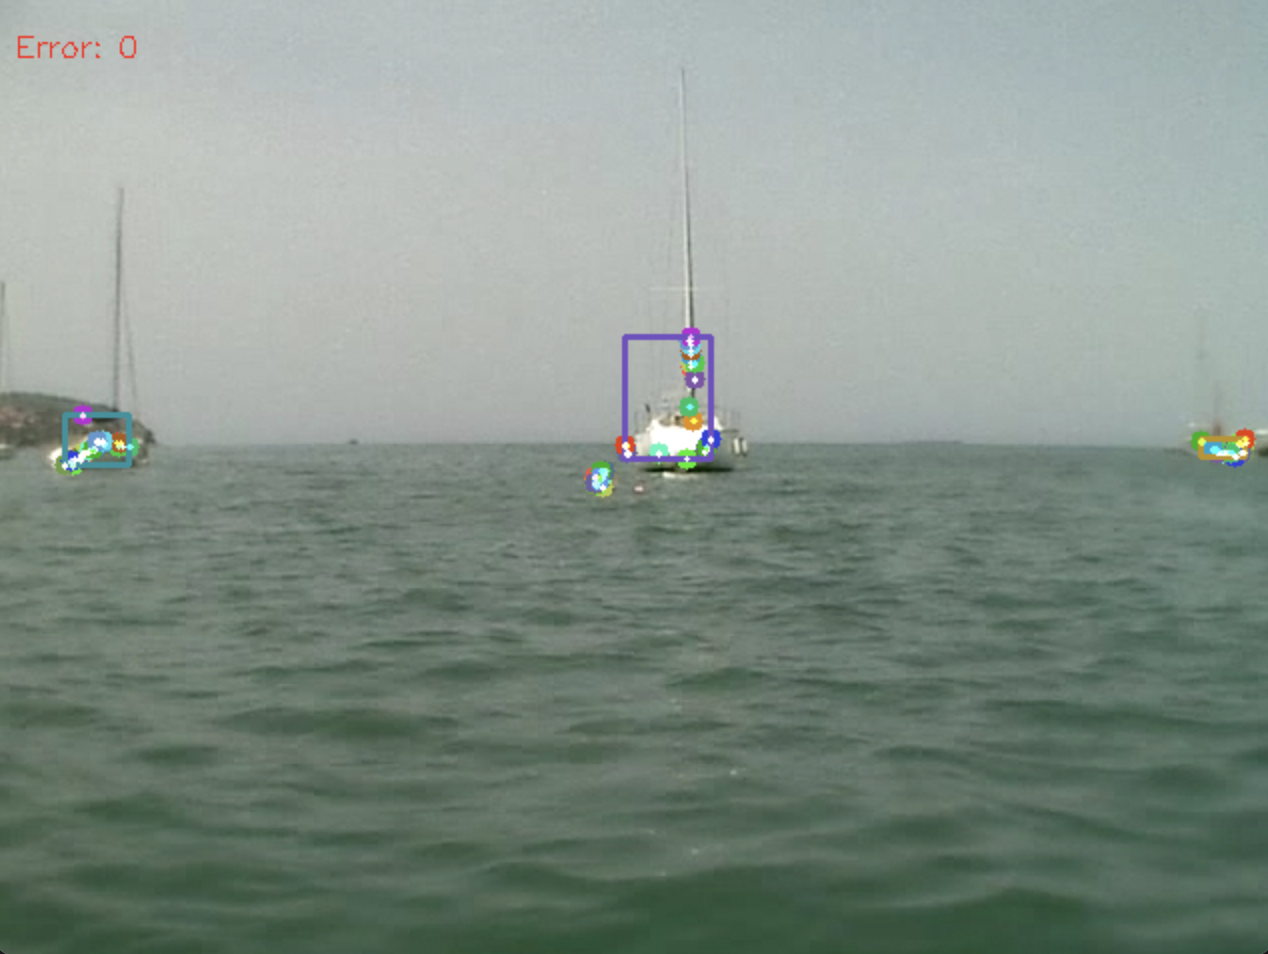
\includegraphics[width=\linewidth]{images/screen_1.png}
   \caption{First frame of a video from MODD. Feature points were calculated using Shi-Tomasi corner
   detector for each object separately. Bounding boxes have also been calculated.}
   \label{fig:first_frame}
\end{figure}

\subsection{Tracking feature points and generating bounding boxes}\label{sofot_bbox}

Tracking of the feature points is done using Lucas-Kanade method for optical flow
estimation \cite{lucas-kanade}. For each set of feature points corresponding to
each of the objects being tracked, a bounding box is calculated. The bounding box is
simply calculated as the smallest rectangle enclosing all the feature points for a
given object. Mathematically, we can present a bounding box as a tuple $B = (P_1, P_2)$,
where $P_i = (x_i, y_i)$, and $P_1$ is the upper left corner and $P_2$ is the lower
right corner of the bounding box. Calculating the bounding box can then be expressed simply as

\begin{equation}
   B_i = \left( \left(\min_{(x,y) \in \mathcal{P}_i} x, \min_{(x,y) \in \mathcal{P}_i} y\right), \left(\max_{(x,y) \in \mathcal{P}_i} x, \max_{(x,y) \in \mathcal{P}_i} y\right) \right),
\end{equation}

where $B_i$ is the bounding box of $i$-th tracked object and $\mathcal{P}_i$ is the
set of feature points used for optical flow estimation of $i$-th tracked object.

It is worth noting, that objects that were present in the old frame and are not present
in the current frame, have an empty set of feature points $\mathcal{P} = \emptyset$.
They are ignored from now on, even if they reappear in some future frame. Figure
\ref{fig:sofot_track} shows feature points' tracks together with current bounding box after a couple of frames.

\begin{figure}
   \centering
   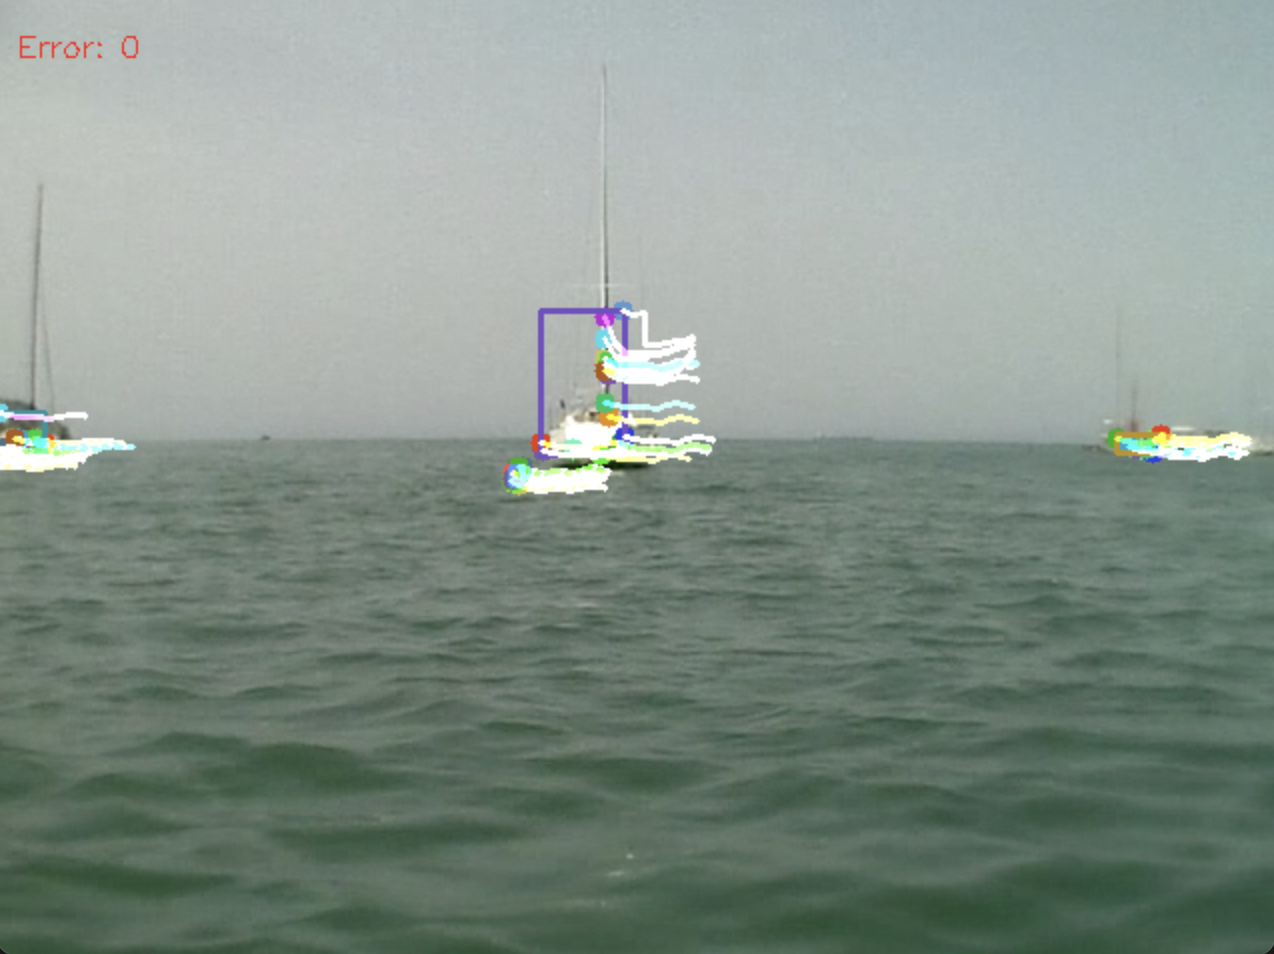
\includegraphics[width=\linewidth]{images/screen_of.png}
   \caption{Feature points' tracks after a couple of frames. Bounding boxes are drawn
   around the newest points as a smallest rectangle enclosing all the feature points.}
   \label{fig:sofot_track}
\end{figure}

\subsection{Object tracking}\label{sofot_track}

Given a set of bounding boxes from previous frame and bounding boxes for current
frame, all that needs to be done in order to actually track the objects is to match
old bounding boxes with the newly generated ones. The matching is described in the following
paragraphs.

First, an intersection over union (IoU) is calculated over cartesian product of
old bounding boxes and new ones. Bounding boxes and therefore objects are paired so that
each old bounding box is mapped to the new one having the highest IoU with that particular
old one. Duplicates are obviously not allowed. In mathematical language we can express this
as

\begin{equation}
   \big(B, \tilde{B}\big) = \left(B, \argmax_{B_{\text{new}}} \iou(B,B_{\text{new}})\right).
\end{equation}

Then, if there are some old bounding boxes that were not matched with new ones, there are two
options. First option is that an object has exited the frame and was ignored in previous step, meaning it
can be left unpaired. Second option is that an object has moved so much from the previous frame
that the new bounding box does not overlap with it anymore. This is extremely unlikely in
steady environments but it has to be taken into account in order to produce a more robust algorithm.
Such old bounding boxes are paired with remaining new bounding boxes so that the distance
between the bounding boxes is the smallest. In mathematical language, this pairing
can be described as

\begin{equation}
   \big(B, \tilde{B}\big) = \left( B, \argmax_{B_{\text{new}}} d(B, B_{\text{new}}) \right),
\end{equation}

where

\begin{multline}
   d(B_1, B_2) =\\ d\left( \big((x_{11}, y_{11}), (x_{12}, y_{12})\big), \big((x_{21}, y_{21}), (x_{22}, y_{22})\big) \right)
\end{multline}

is a distance function defined as

\begin{multline}
   d(B_1, B_2) =\\ \min\{ |x_{11} - x_{22}|, |y_{11} - y_{22}|, |x_{12} - x_{21}|, |y_{12} - y_{21}| \}.
\end{multline}

After this step, all old bounding boxes have a corresponding new bounding box, or they have exited the frame.
This concludes the tracking step.

\subsection{Gluing pieces together}

Algorithm is initialised with the step provided in \ref{sofot_init}. Then, the algorithm
iterates over all given frames executing operations described in \ref{sofot_bbox} and \ref{sofot_track}.
The output of the algorithm are bounding boxes of obstacles tracked for each frame. Algorithm
can save the bounding boxes for each frame to separate file if so desired.

\subsection{Measuring error}

The error is defined as the number of frames that contain a bounding box generated by SOFOT that
does not overlap with any of the ground-truth bounding boxes.
In order to measure error, a ground-truth annotations of bounding boxes must therefore be fed into SOFOT.
This measure for the error is justified by the fact that it represents wrong detections, i.e. detections
that are either not in the ground-truth annotations or detections that are misplaced from ground-truth.
Detections that are in ground-truth annotations and are missing in SOFOT detections can be ignored
due to the fact that SOFOT only tracks objects until they go out of frame for the first time. This means
that if an object reappears in the scene, SOFOT ignores it and this is not an error. This process of forgetting
is shown and described in greater detail in figure \ref{fig:sofot_out_of_frame}.

\begin{figure}
   \centering
   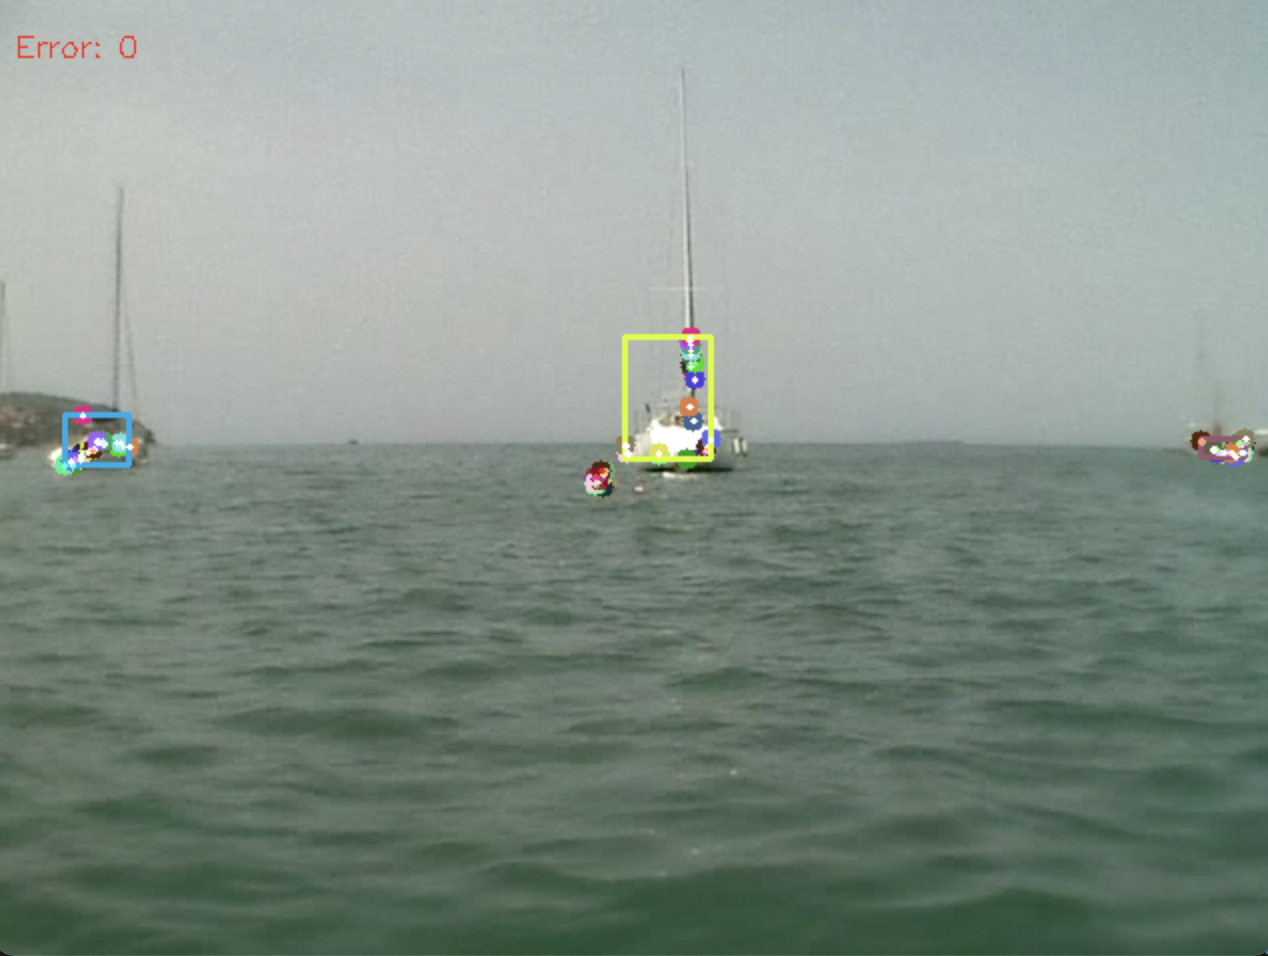
\includegraphics[width=\linewidth]{images/forgetting1.png}
   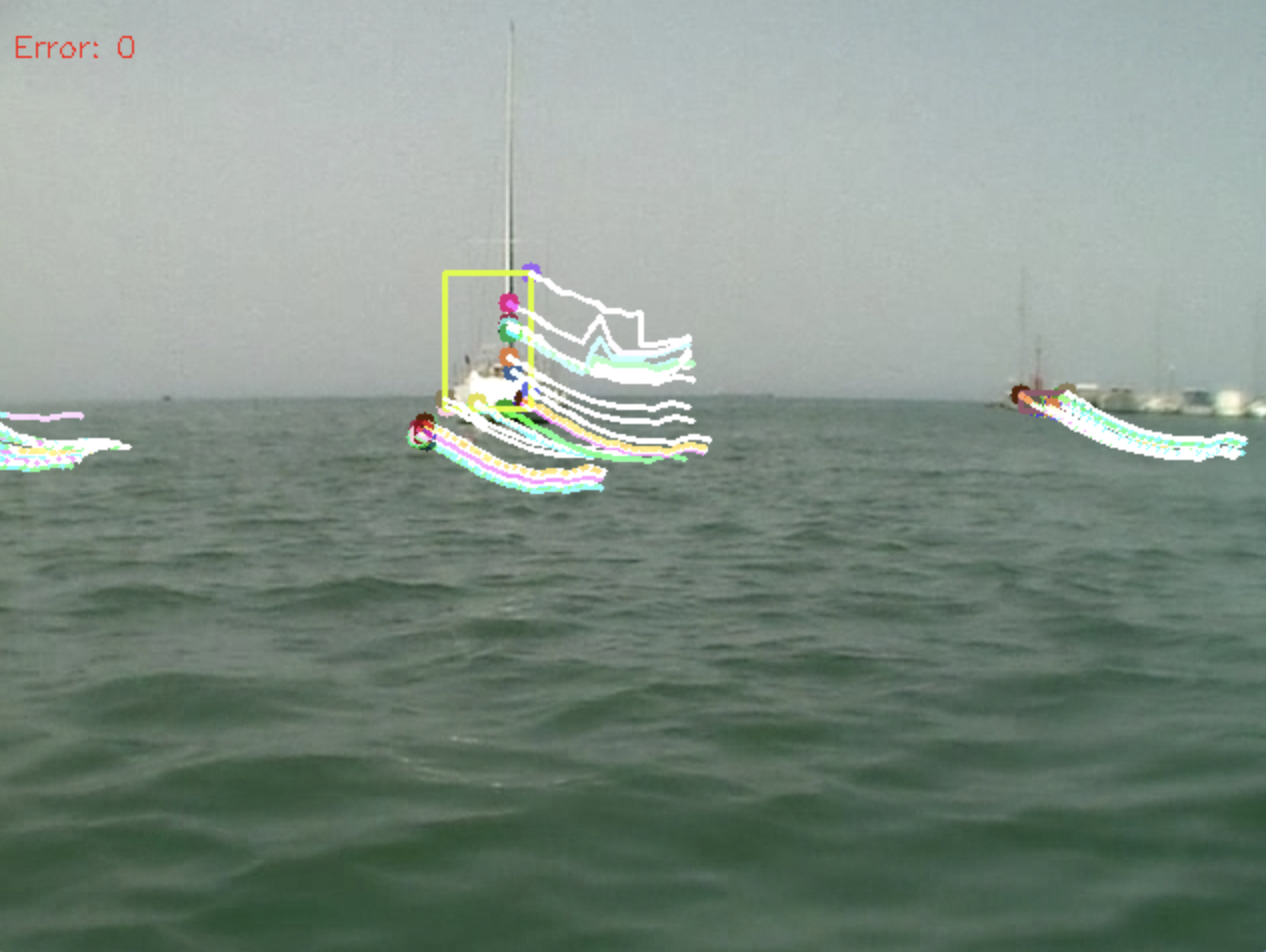
\includegraphics[width=\linewidth]{images/forgetting2.png}
   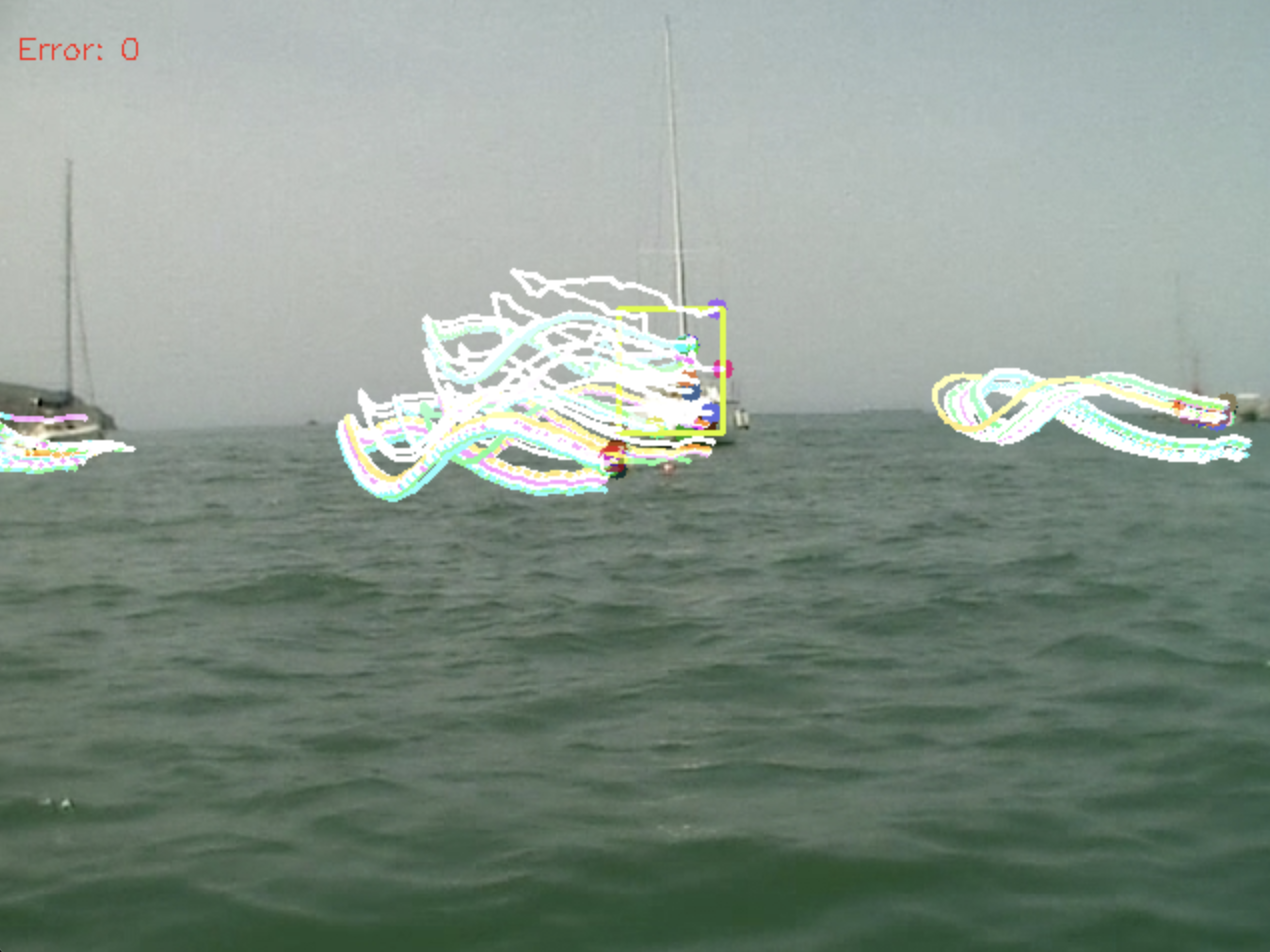
\includegraphics[width=\linewidth]{images/forgetting3.png}
   \caption{Forgetting of the object, the only "flaw" of SOFOT. At the start (upper image), there were
   given four object detections. After some time (middle image), the sailing boat on the left (marked with blue in the upper image)
   disappeared from the scene. More time passed and the blue-marked sailing boat appeared in the scene again,
   however due to forgetting nature of SOFOT it was not tracked anymore. We left the possible improvements regarding
   this flaw for future work (see \ref{sec:future_work}).}
   \label{fig:sofot_out_of_frame}
\end{figure}


%%%%%%%%%%%%%%%%%%%%%%%%%%%%%%%%%%%%%%%%%%%%%%%%%%%%%%%%%%%%%%%%%%%%%%%%%%%%%%%%%%%%%%%%%%%%%%%%
%%%%%%%%%%%%%%%%%%%%%%%%%%%%%%%%%%%%%%%%%%%%%%%%%%%%%%%%%%%%%%%%%%%%%%%%%%%%%%%%%%%%%%%%%%%%%%%%
%%%%%%%%%
%%%%%%%%% RESULTS
%%%%%%%%%
%%%%%%%%%%%%%%%%%%%%%%%%%%%%%%%%%%%%%%%%%%%%%%%%%%%%%%%%%%%%%%%%%%%%%%%%%%%%%%%%%%%%%%%%%%%%%%%%
%%%%%%%%%%%%%%%%%%%%%%%%%%%%%%%%%%%%%%%%%%%%%%%%%%%%%%%%%%%%%%%%%%%%%%%%%%%%%%%%%%%%%%%%%%%%%%%%

\section{Experiments and Results}

We have tested SOFOT on Marine Obstacle Detection Dataset (MODD) \cite{kristan2015fast,kristan2014graphical}.
The dataset consists of 12 videos in maritime environment, captured by USV. The videos in dataset
are taken under different conditions, in normal lighting, low lighting, and extreme sunlight,
rendering the MODD a good dataset for benchmarking and testing SOFOT, which was made for steady environments
like maritime.

We have benchmarked the frames-per-second (FPS) processed by SOFOT for each video in the dataset
and the results are presented in great detail in table \ref{tab:results}. The average FPS over
all videos was 213, which gives more than enough breathing area for post-processing of detections,
such as usage of bounding boxes in collision prevention or path-finding algorithms.
The benchmarks were run on a single core of Intel i9-9980HK with base frequency of $2.4\,\text{GHz}$.


\begin{table}
   \centering
   \begin{tabular}{c|c|c}
      \textbf{video} & \textbf{FPS} & \textbf{error (at frame)}\\\hline
      01 & 144 & 0\\
      02 & 233 & 0\\
      03 & 162 & 0\\
      04 & 240 & 0\\
      05 & 233 & 0\\
      06 & 227 & 0\\
      07 & 245 & 0\\
      08 & 238 & 0\\
      09 & 180 & 1 (108/108)\\
      10 & 186 & 0\\
      11 & 238 & 0\\
      12 & 233 & 0\\\hline
      average & 213 & 0
   \end{tabular}
   \caption{Frames-per-second (FPS) processed by SOFOT and number of errors with the number of
   frame of first error encountered for Marine Obstacle Detection Dataset (MODD). The average
   FPS clearly leaves enough breathing room for further processing of generated bounding boxes
   by a path-finding or collision prevention systems. As seen in the error column, SOFOT managed
   to track all objects appearing on the first frame until they either exited the frame for the first
   time or until the end. The only error was made in the last frame of video 09, and the reason
   for the error is that all features of the object that SOFOT tracked exited the video on frame 108,
   thus resulting in object not being ignored, although part of the object was still visible on frame.}
   \label{tab:results}
\end{table}


%%%%%%%%%%%%%%%%%%%%%%%%%%%%%%%%%%%%%%%%%%%%%%%%%%%%%%%%%%%%%%%%%%%%%%%%%%%%%%%%%%%%%%%%%%%%%%%%
%%%%%%%%%%%%%%%%%%%%%%%%%%%%%%%%%%%%%%%%%%%%%%%%%%%%%%%%%%%%%%%%%%%%%%%%%%%%%%%%%%%%%%%%%%%%%%%%
%%%%%%%%%
%%%%%%%%% FUTURE WORK
%%%%%%%%%
%%%%%%%%%%%%%%%%%%%%%%%%%%%%%%%%%%%%%%%%%%%%%%%%%%%%%%%%%%%%%%%%%%%%%%%%%%%%%%%%%%%%%%%%%%%%%%%%
%%%%%%%%%%%%%%%%%%%%%%%%%%%%%%%%%%%%%%%%%%%%%%%%%%%%%%%%%%%%%%%%%%%%%%%%%%%%%%%%%%%%%%%%%%%%%%%%

\section{Future Work}\label{sec:future_work}

SOFOT has a great potential to be upgraded and integrated into different systems.

One possible upgrade is the possibility to track objects that are not present on the
first frame of the video but appear on camera later on. This would bring SOFOT way closer
to production-ready software. Another similar upgrade is the ability to reidentify
the objects that once left the frame and reappeared back on frame later on. The reidentification
is however not essential, and the aforementioned upgrade is completely satisfactory.

Another possible upgrade is to support multiple cameras, opening the way to integrating
position estimation right into SOFOT. Even better option is to support 360-degree cameras,
preventing a close object to ever getting out of frame. This would allow collision
prevention system to run with lighter or completely without algorithms for path prediction
of obstacles, thus making the unmanned vehicle more secure.

Currently, bounding boxes of the objects are a mere and quite imprecise estimation of the true
bounding box. Current implementation of bounding box calculation is this naive to provide much faster execution
times. This leads to another opportunity for future improvements, that being a better and
more precise bounding box calculation, if and only if it does not impact the running
time too much. All in all, one has to remember that near-perfect bounding box is completely
unnecessary for unmanned aerial and surface vehicles, because the obstacles in target environments
of these two types of machines should be avoided by a great distance. This means, that the error
in bounding box calculation should be negligible compared to evading distance.


%%%%%%%%%%%%%%%%%%%%%%%%%%%%%%%%%%%%%%%%%%%%%%%%%%%%%%%%%%%%%%%%%%%%%%%%%%%%%%%%%%%%%%%%%%%%%%%%
%%%%%%%%%%%%%%%%%%%%%%%%%%%%%%%%%%%%%%%%%%%%%%%%%%%%%%%%%%%%%%%%%%%%%%%%%%%%%%%%%%%%%%%%%%%%%%%%
%%%%%%%%%
%%%%%%%%% CONCLUSION
%%%%%%%%%
%%%%%%%%%%%%%%%%%%%%%%%%%%%%%%%%%%%%%%%%%%%%%%%%%%%%%%%%%%%%%%%%%%%%%%%%%%%%%%%%%%%%%%%%%%%%%%%%
%%%%%%%%%%%%%%%%%%%%%%%%%%%%%%%%%%%%%%%%%%%%%%%%%%%%%%%%%%%%%%%%%%%%%%%%%%%%%%%%%%%%%%%%%%%%%%%%

\section{Conclusion}

The method for object tracking presented in this work turned out to be insanely fast
and accurate, thus making it very usable in systems with limited computer power, such as
autonomous vehicles. The only assumption SOFOT depends on is that the environment is
somewhat steady, without rapid one-frame time period changes. Given the targeted environments
and the fact that cameras with normal frame rates are widely available, this is a sane and
justifiable assumption. We think, that SOFOT is near-production-ready even without
improvements mentioned in section \ref{sec:future_work}, although they would be a really-nice-to-have.
and a graphical user interface would be a cherry on top.


%%%%%%%%%%%%%%%%%%%%%%%%%%%%%%%%%%%%%%%%%%%%%%%%%%%%%%%%%%%%%%%%%%%%%%%%%%%%%%%%%%%%%%%%%%%%%%%%
%%%%%%%%%%%%%%%%%%%%%%%%%%%%%%%%%%%%%%%%%%%%%%%%%%%%%%%%%%%%%%%%%%%%%%%%%%%%%%%%%%%%%%%%%%%%%%%%
%%%%%%%%%
%%%%%%%%% BIBLIOGRAPHY
%%%%%%%%%
%%%%%%%%%%%%%%%%%%%%%%%%%%%%%%%%%%%%%%%%%%%%%%%%%%%%%%%%%%%%%%%%%%%%%%%%%%%%%%%%%%%%%%%%%%%%%%%%
%%%%%%%%%%%%%%%%%%%%%%%%%%%%%%%%%%%%%%%%%%%%%%%%%%%%%%%%%%%%%%%%%%%%%%%%%%%%%%%%%%%%%%%%%%%%%%%%

{\small
\bibliographystyle{ieee_fullname}
\bibliography{egbib}
}

\end{document}
